\section{Results}

\subsection{Proof of convergence history}
Pleas see Appendix
\subsection{Table of final lift and drag coefficients and related forces}
\begin{table}[H]
	\centering
	\begin{tabular}{|c|c|c|c|c|} \hline
		\centering
		\textbf{Case [$^\circ$]} & $C_L$ [-]   & $C_D$ [-]   & Lift [N] & Drag [N]  \\ \hline
		10         & 0.143 & 0.075 & 405,550 & 212,700\\ \hline
		20         & 0.341 & 0.174 & 967,090 & 493,470\\ \hline
		30         & 0.545 & 0.371 & 1,545,600 & 1,052,200\\ \hline
	\end{tabular}
\end{table}

\subsection{Plot of lift and drag and L/D vs. AOA with peak L/D identified}

\begin{figure}[H]
 \centering
 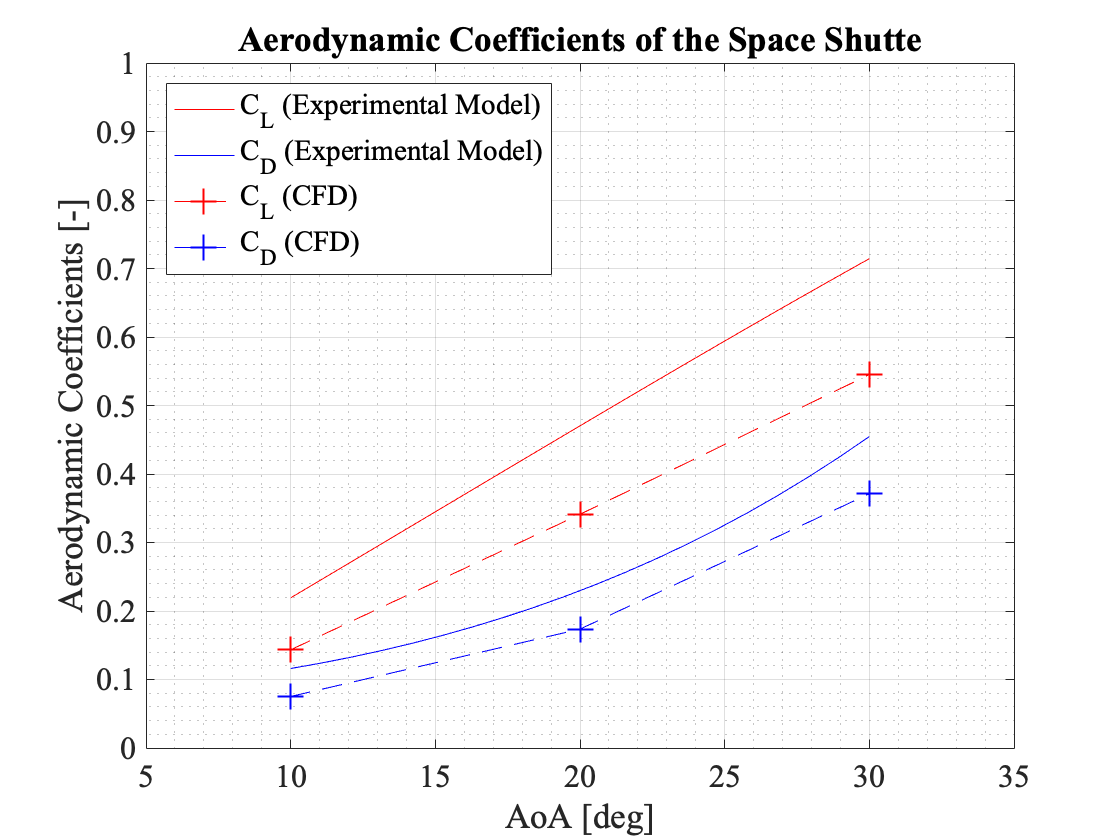
\includegraphics[width=0.7\textwidth]{matlab_images/aero_coeff_comp.png}
 \caption{Comparison of the $C_L$ and $C_D$ results from the experimental model and the CFD cases ran}
 \label{fig: aero_coeff_comp}
\end{figure}

\begin{figure}[H]
 \centering
 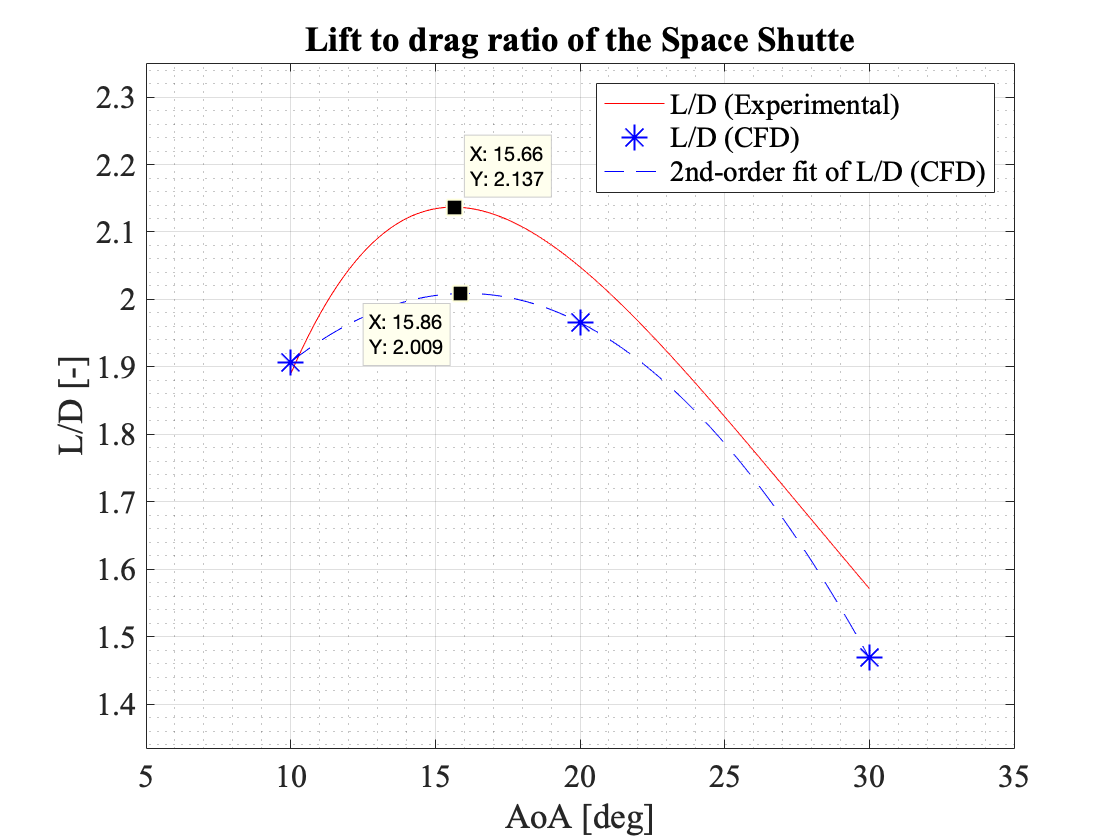
\includegraphics[width=0.7\textwidth]{matlab_images/L2D.png}
 \caption{Comparison of the lift-to-drag ratios from the experimental model and the CFD cases ran}
 \label{fig: l2d}
\end{figure}

\subsection{Pressure and temperature contours with streamlines}

\subsubsection{AoA = 10$^\circ$}
\begin{figure}[H]

	\centering
    \begin{subfigure}[b]{0.65\textwidth}
         \centering
		 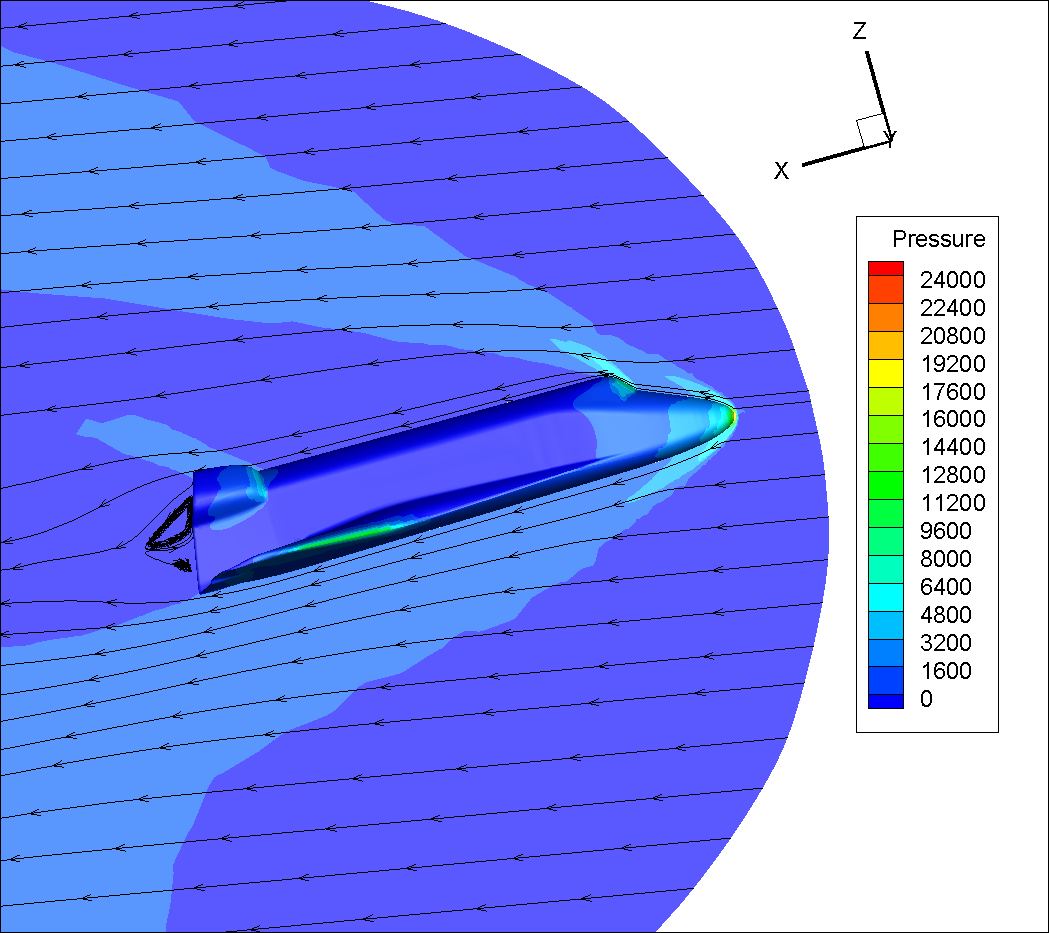
\includegraphics[width=\textwidth]{report_images/10_sym_pressure_contour.png}
		 \caption{Pressure contour at the symmetry plane of the orbiter at 10 degs AoA}
		 \label{fig: 10_sym_pressure_contour}
    \end{subfigure} 
    \begin{subfigure}[b]{0.65\textwidth}
         \centering
		 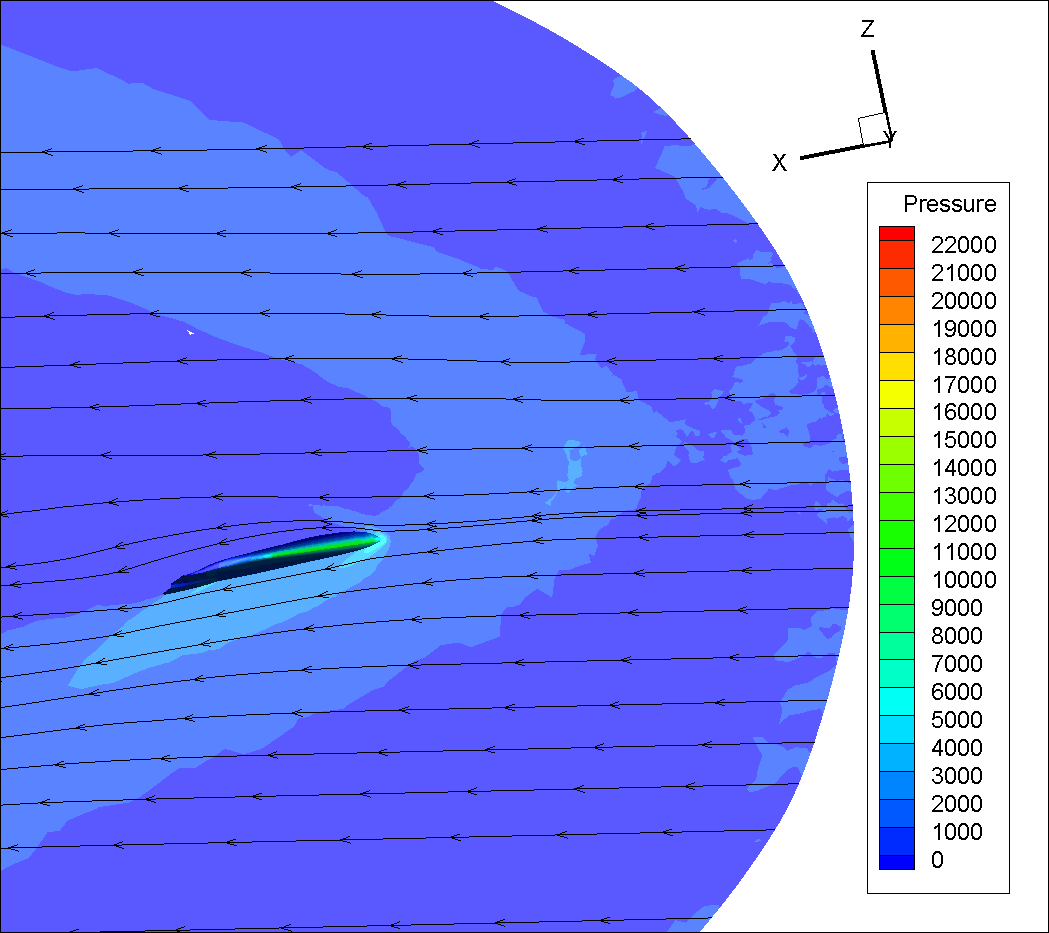
\includegraphics[width=\textwidth]{report_images/10_wing_pressure_contour.png}
		 \caption{Pressure contour at the midspan of the wing of the orbiter at 10 degs AoA}
		 \label{fig: 10_wing_pressure_contour}
    \end{subfigure}
%	\caption{Caption place holder}  
\end{figure}

\begin{figure}[H]

	\centering
    \begin{subfigure}[b]{0.65\textwidth}
         \centering
		 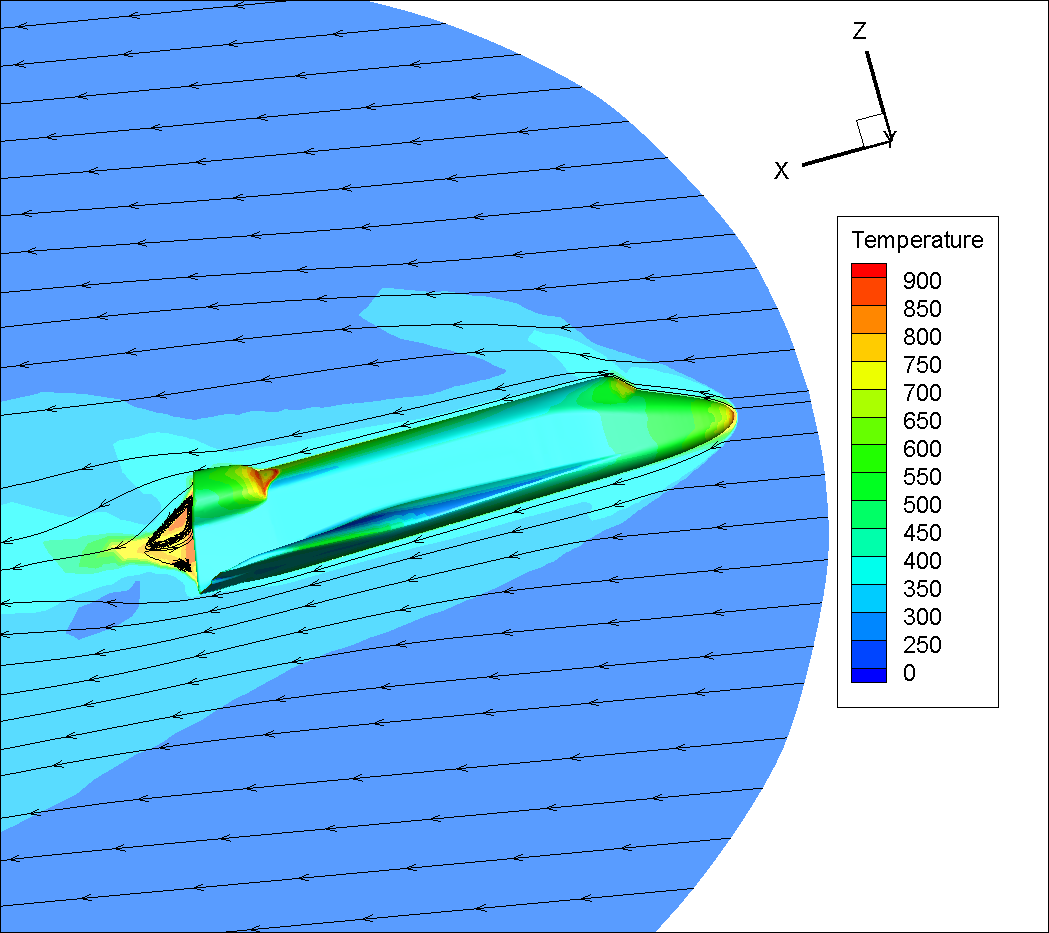
\includegraphics[width=\textwidth]{report_images/10_sym_temp_contour.png}
		 \caption{Temperature contour at the symmetry plane of the orbiter at 10 degs AoA}
		 \label{fig: 10_sym_temp_contour}
    \end{subfigure} 
    \begin{subfigure}[b]{0.65\textwidth}
         \centering
		 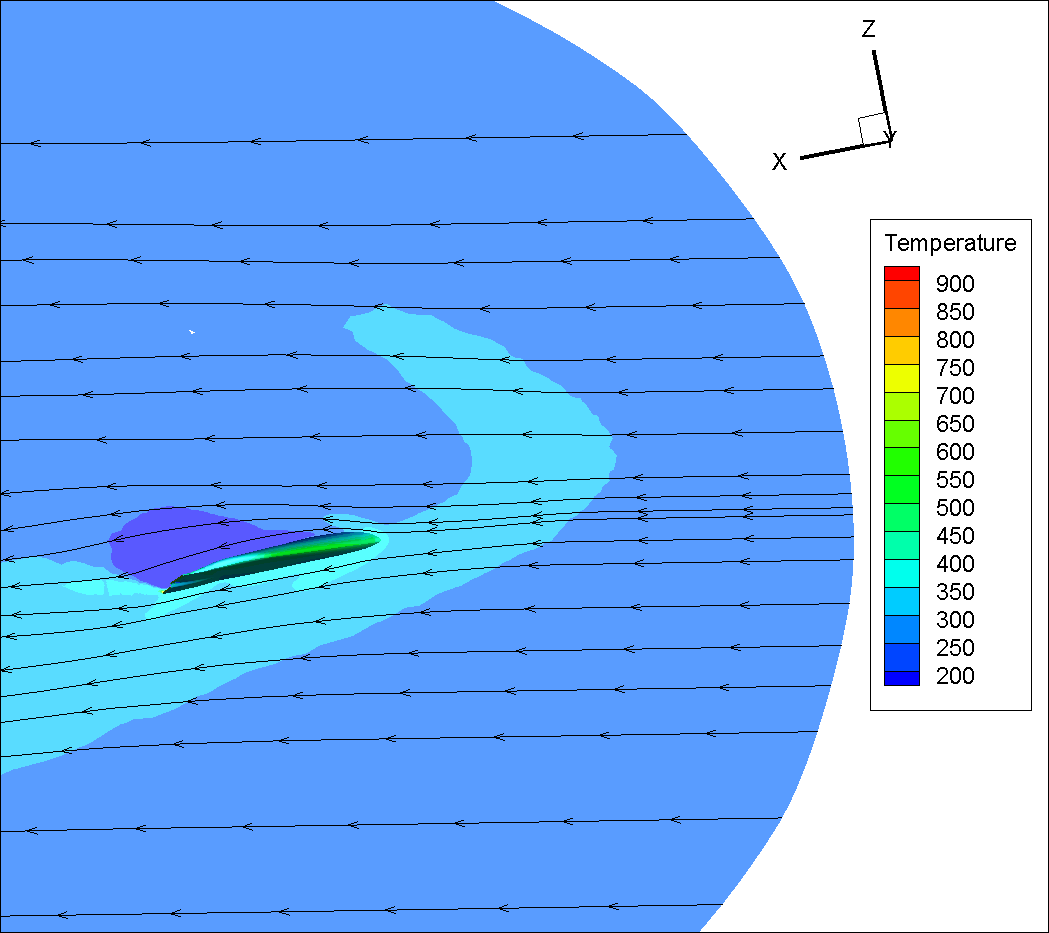
\includegraphics[width=\textwidth]{report_images/10_wing_temp_contour.png}
		 \caption{Temperature contour at the midspan of the wing of the orbiter at 10 degs AoA}
		 \label{fig: 10_wing_temp_contour}
    \end{subfigure}
%	\caption{Caption place holder}  
\end{figure}

\subsubsection{AoA = 20$^\circ$}
\begin{figure}[H]

	\centering
    \begin{subfigure}[b]{0.65\textwidth}
         \centering
		 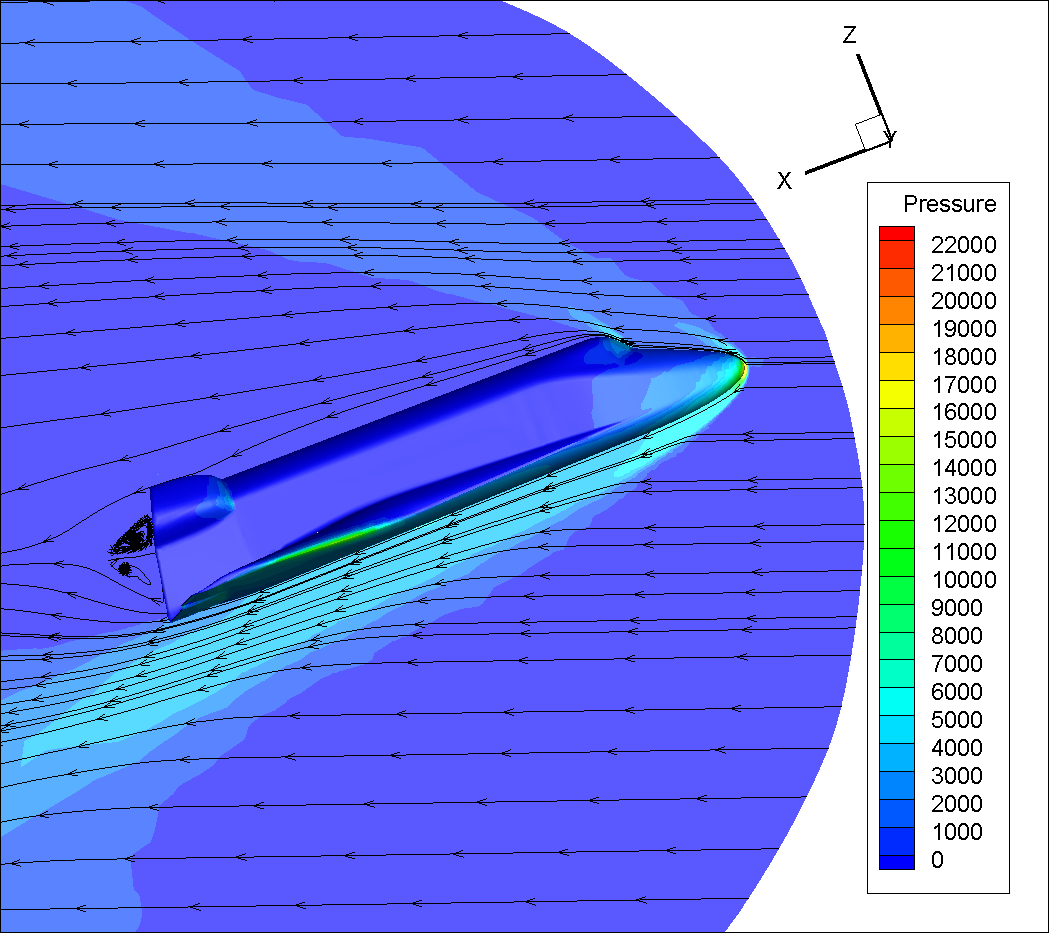
\includegraphics[width=\textwidth]{report_images/20_sym_pressure_contour.png}
		 \caption{Pressure contour at the symmetry plane of the orbiter at 20 degs AoA}
		 \label{fig: 20_sym_pressure_contour}
    \end{subfigure} 
    \begin{subfigure}[b]{0.65\textwidth}
         \centering
		 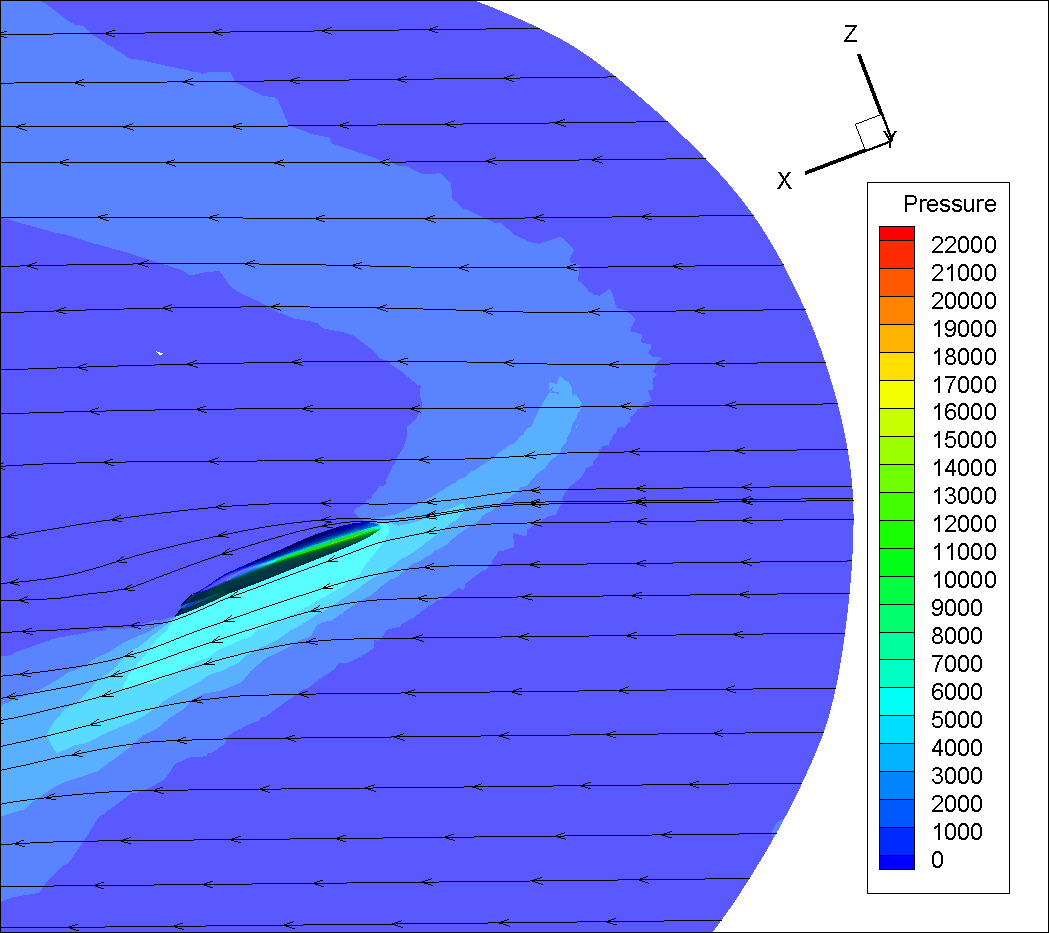
\includegraphics[width=\textwidth]{report_images/20_wing_pressure_contour.png}
		 \caption{Pressure contour at the midspan of the wing of the orbiter at 20 degs AoA}
		 \label{fig: 20_wing_pressure_contour}
    \end{subfigure}
%	\caption{Caption place holder}  
\end{figure}

\begin{figure}[H]

	\centering
    \begin{subfigure}[b]{0.65\textwidth}
         \centering
		 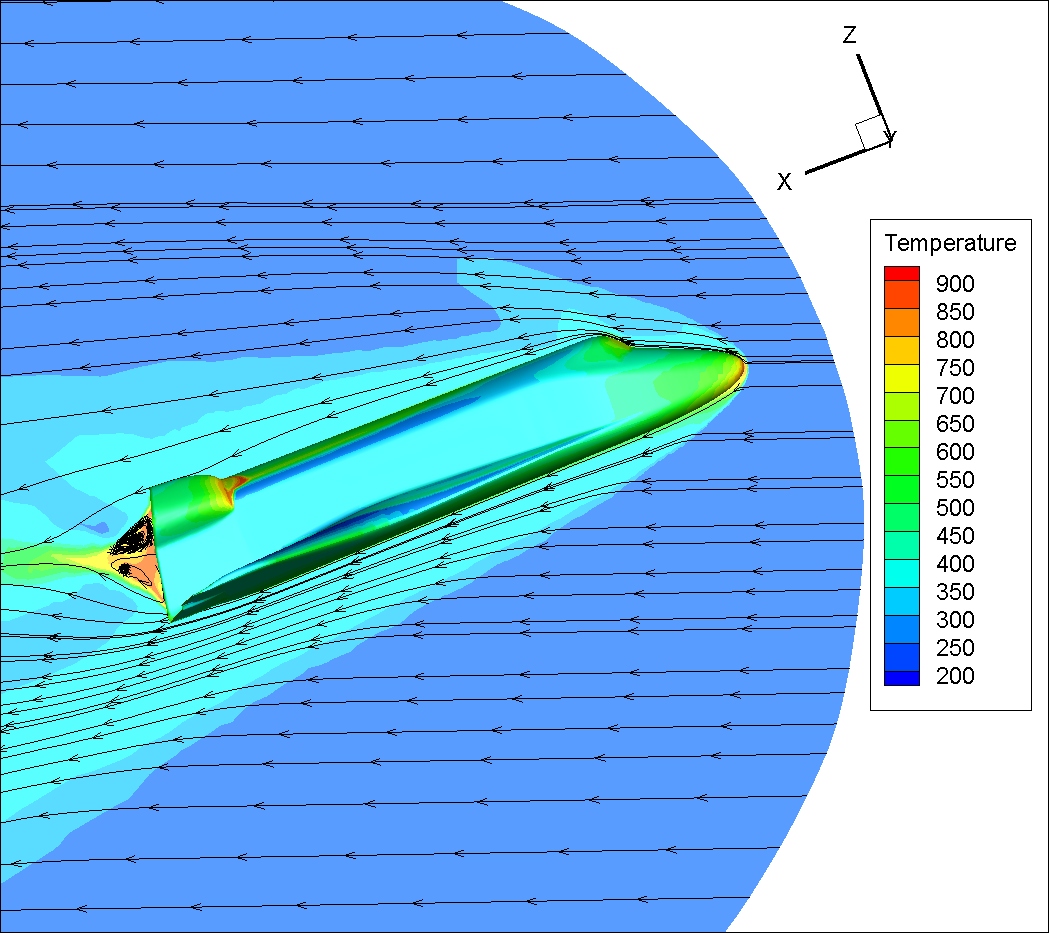
\includegraphics[width=\textwidth]{report_images/20_sym_temp_contour.png}
		 \caption{Temperature contour at the symmetry plane of the orbiter at 20 degs AoA}
		 \label{fig: 20_sym_temp_contour}
    \end{subfigure} 
    \begin{subfigure}[b]{0.65\textwidth}
         \centering
		 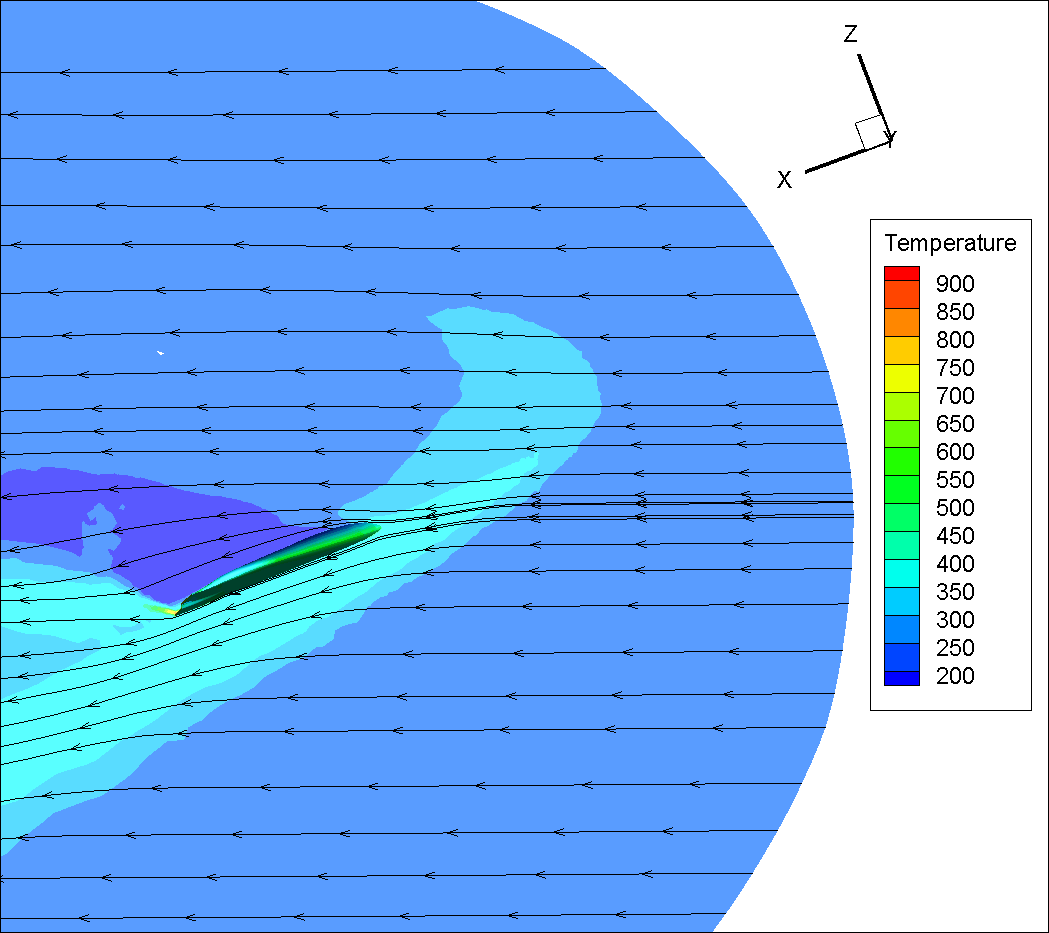
\includegraphics[width=\textwidth]{report_images/20_wing_temp_contour.png}
		 \caption{Temperature contour at the midspan of the wing of the orbiter at 20 degs AoA}
		 \label{fig: 20_wing_temp_contour}
    \end{subfigure}
%	\caption{Caption place holder}  
\end{figure}

\subsubsection{AoA = 30$^\circ$}

\begin{figure}[H]

	\centering
    \begin{subfigure}[b]{0.65\textwidth}
         \centering
		 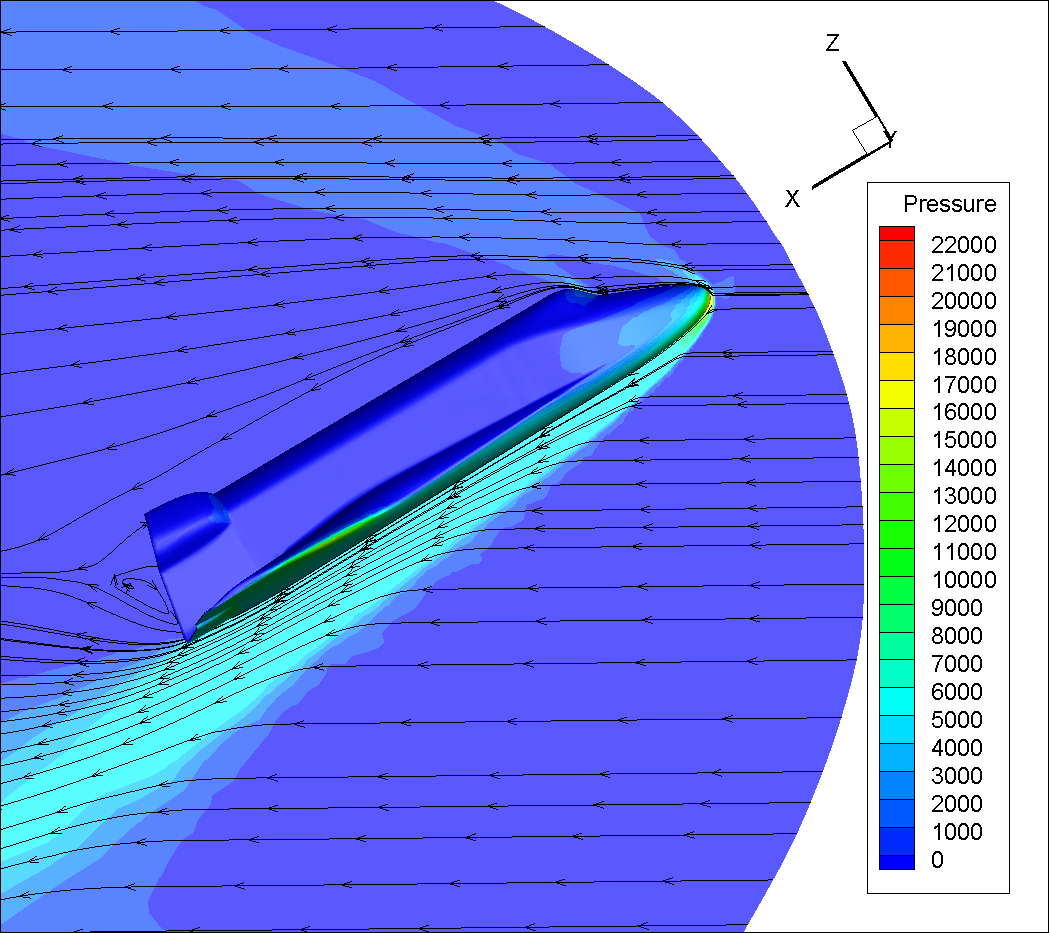
\includegraphics[width=\textwidth]{report_images/30_sym_pressure_contour.png}
		 \caption{Pressure contour at the symmetry plane of the orbiter at 30 degs AoA}
		 \label{fig: 30_sym_pressure_contour}
    \end{subfigure} 
    \begin{subfigure}[b]{0.65\textwidth}
         \centering
		 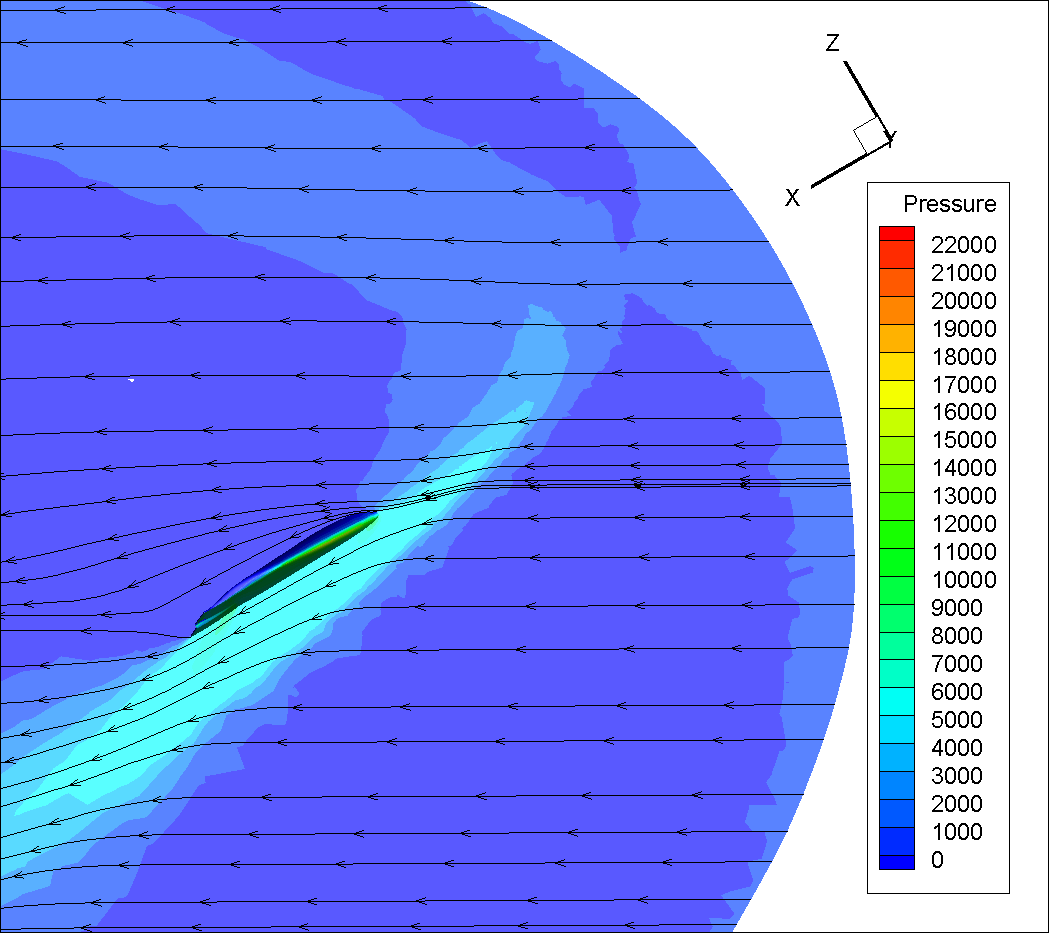
\includegraphics[width=\textwidth]{report_images/30_wing_pressure_contour.png}
		 \caption{Pressure contour at the midspan of the wing of the orbiter at 30 degs AoA}
		 \label{fig: 30_wing_pressure_contour}
    \end{subfigure}
%	\caption{Caption place holder}  
\end{figure}

\begin{figure}[H]

	\centering
    \begin{subfigure}[b]{0.65\textwidth}
         \centering
		 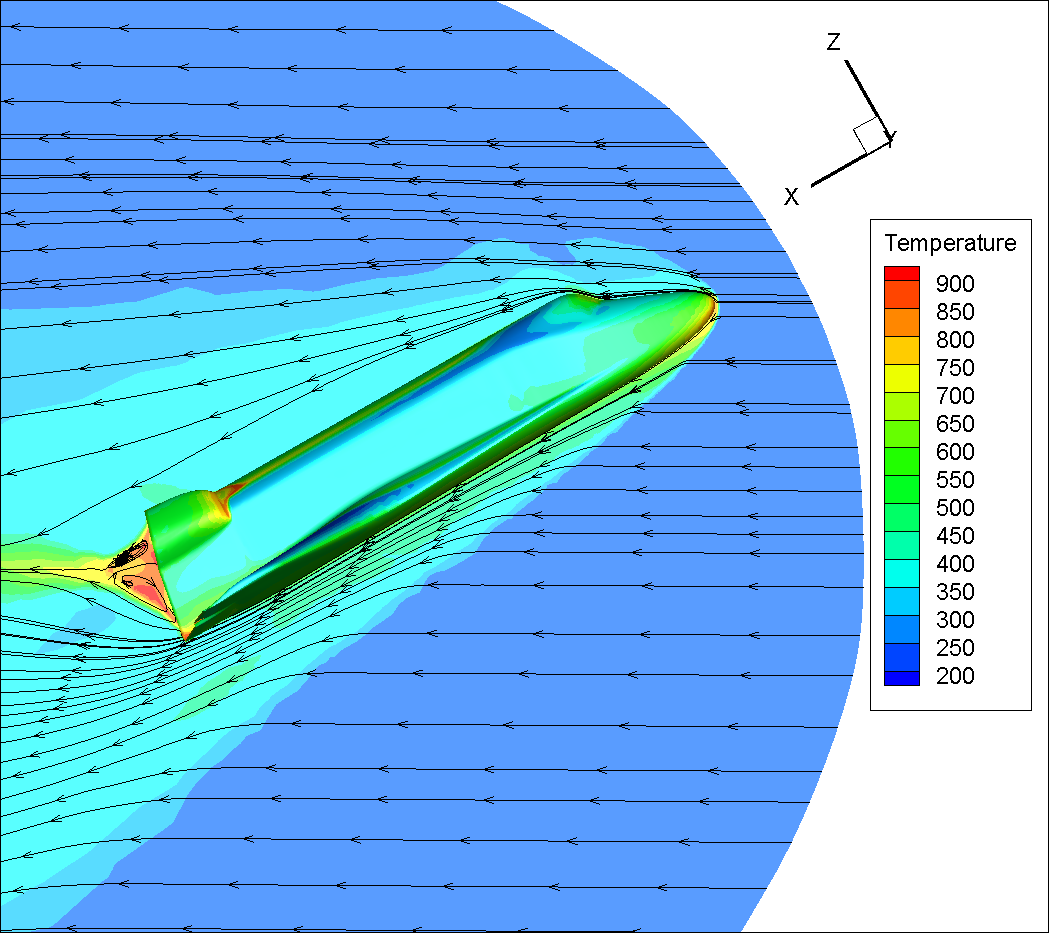
\includegraphics[width=\textwidth]{report_images/30_sym_temp_contour.png}
		 \caption{Temperature contour at the symmetry plane of the orbiter at 30 degs AoA}
		 \label{fig: 30_sym_temp_contour}
    \end{subfigure} 
    \begin{subfigure}[b]{0.65\textwidth}
         \centering
		 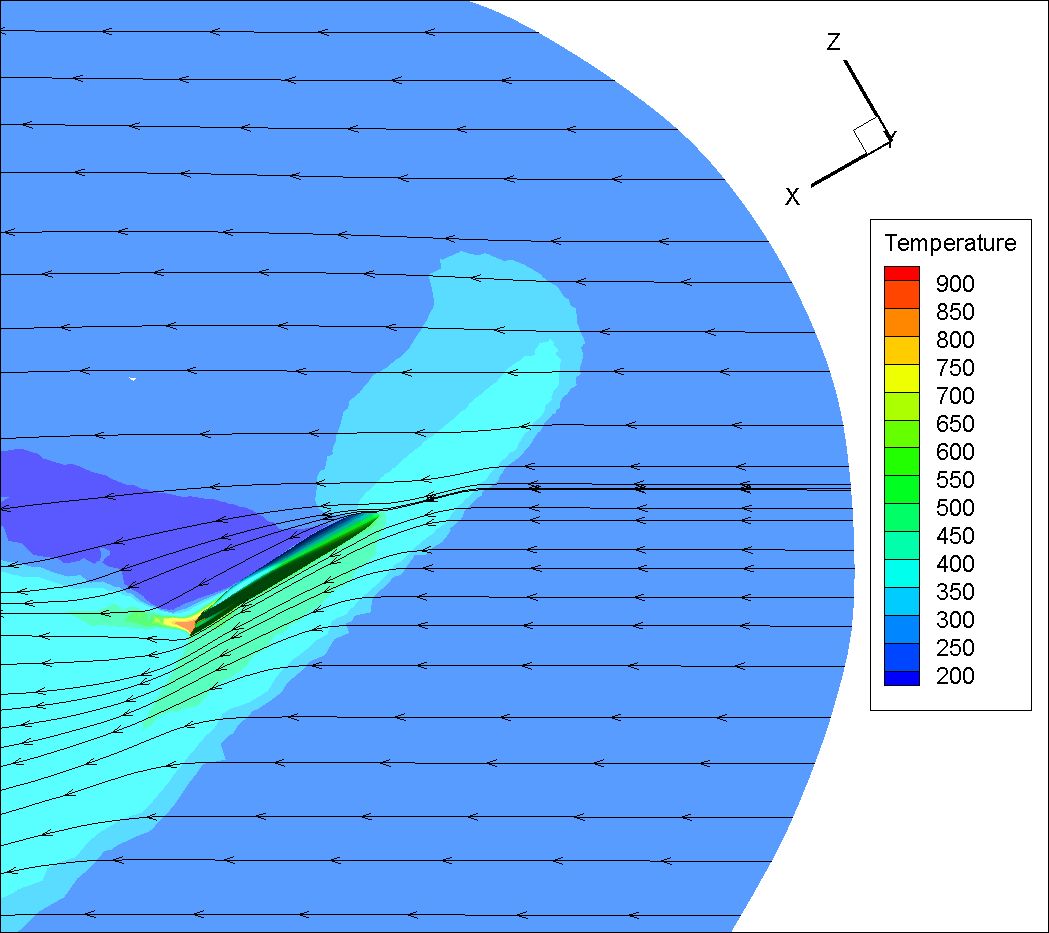
\includegraphics[width=\textwidth]{report_images/30_wing_temp_contour.png}
		 \caption{Temperature contour at the midspan of the wing of the orbiter at 30 degs AoA}
		 \label{fig: 30_wing_temp_contour}
    \end{subfigure}
%	\caption{Caption place holder}  
\end{figure}

\subsection{Results of grid adaptation}

\subsubsection{Side by side of contour plots}
\begin{figure}[H]

	\centering
    \begin{subfigure}[b]{0.65\textwidth}
         \centering
		 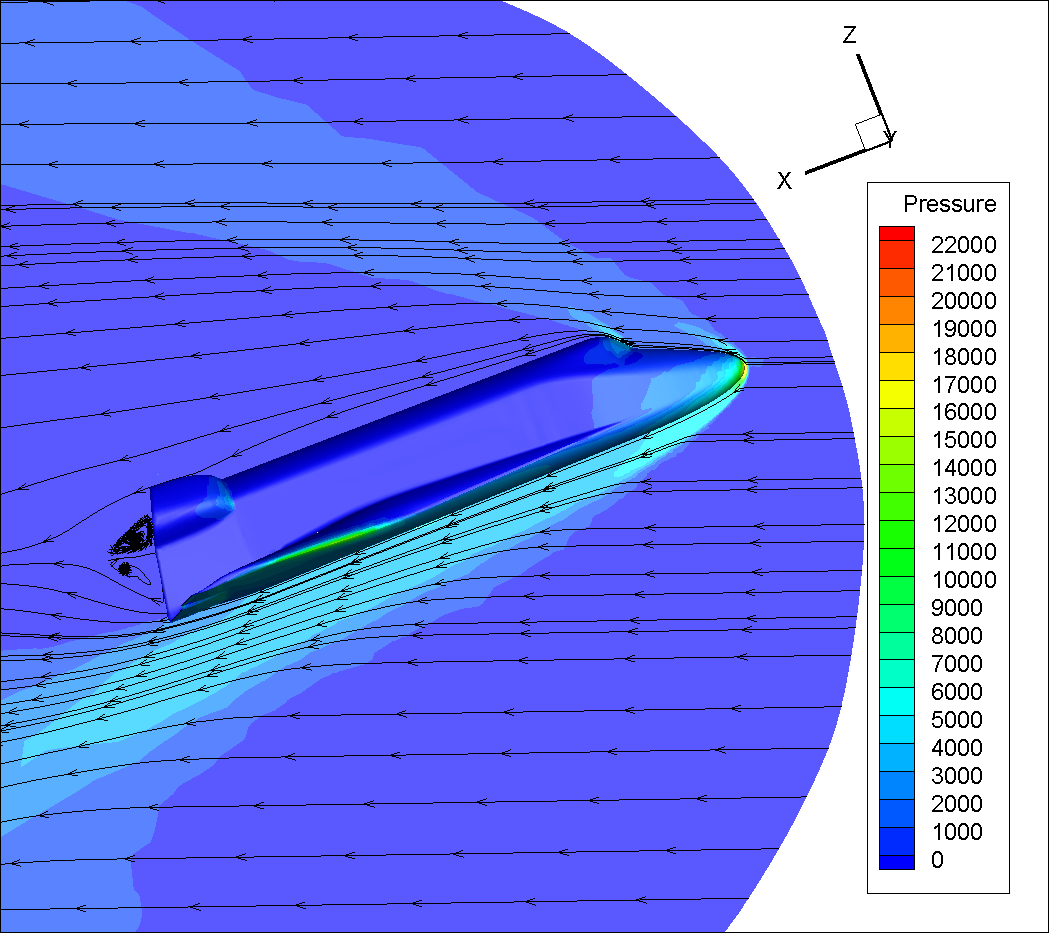
\includegraphics[width=\textwidth]{report_images/20_sym_pressure_contour.png}
		 \caption{Pressure contour at the symmetry plane of the orbiter at 20 degs AoA}
		 \label{fig: 20_sym_pressure_contour}
    \end{subfigure} 
    \begin{subfigure}[b]{0.65\textwidth}
         \centering
		 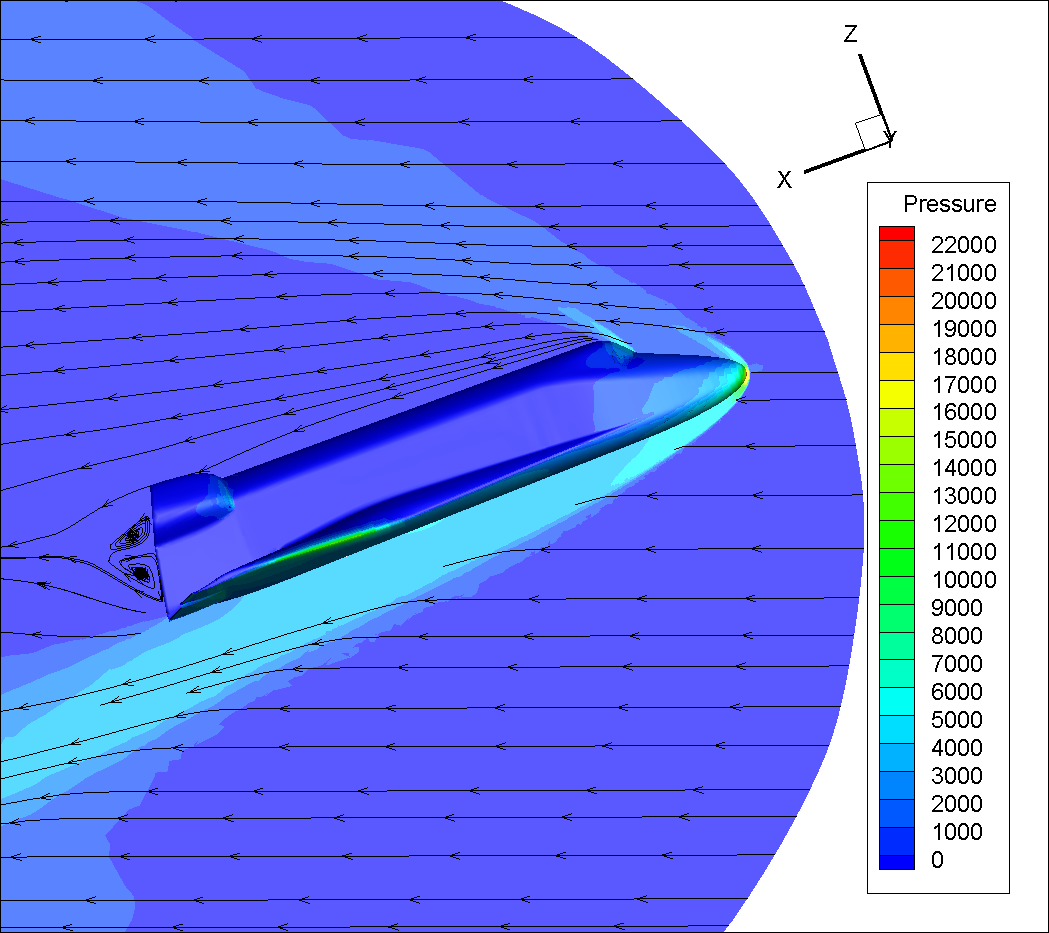
\includegraphics[width=\textwidth]{report_images/20_adapted_sym_pressure_contour.png}
		 \caption{Pressure contour at the symmetry plane of the orbiter at 20 degs AoA using adapted grid}
		 \label{fig: 20_adapt_sym_pressure_contour}
    \end{subfigure}
\end{figure}

\begin{figure}[H]

	\centering
    \begin{subfigure}[b]{0.65\textwidth}
         \centering
		 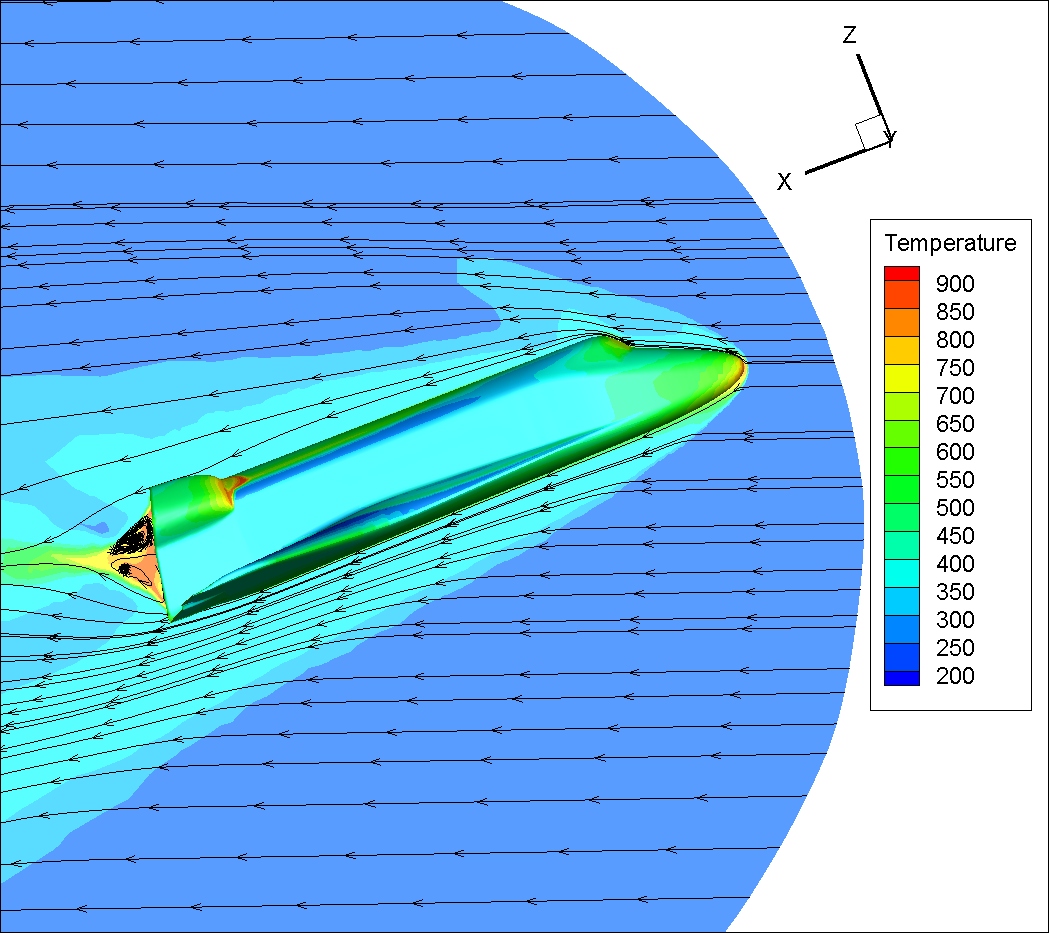
\includegraphics[width=\textwidth]{report_images/20_sym_temp_contour.png}
		 \caption{Temperature contour at the symmetry plane of the orbiter at 20 degs AoA}
		 \label{fig: 20_sym_temp_contour}
    \end{subfigure} 
    \begin{subfigure}[b]{0.65\textwidth}
         \centering
		 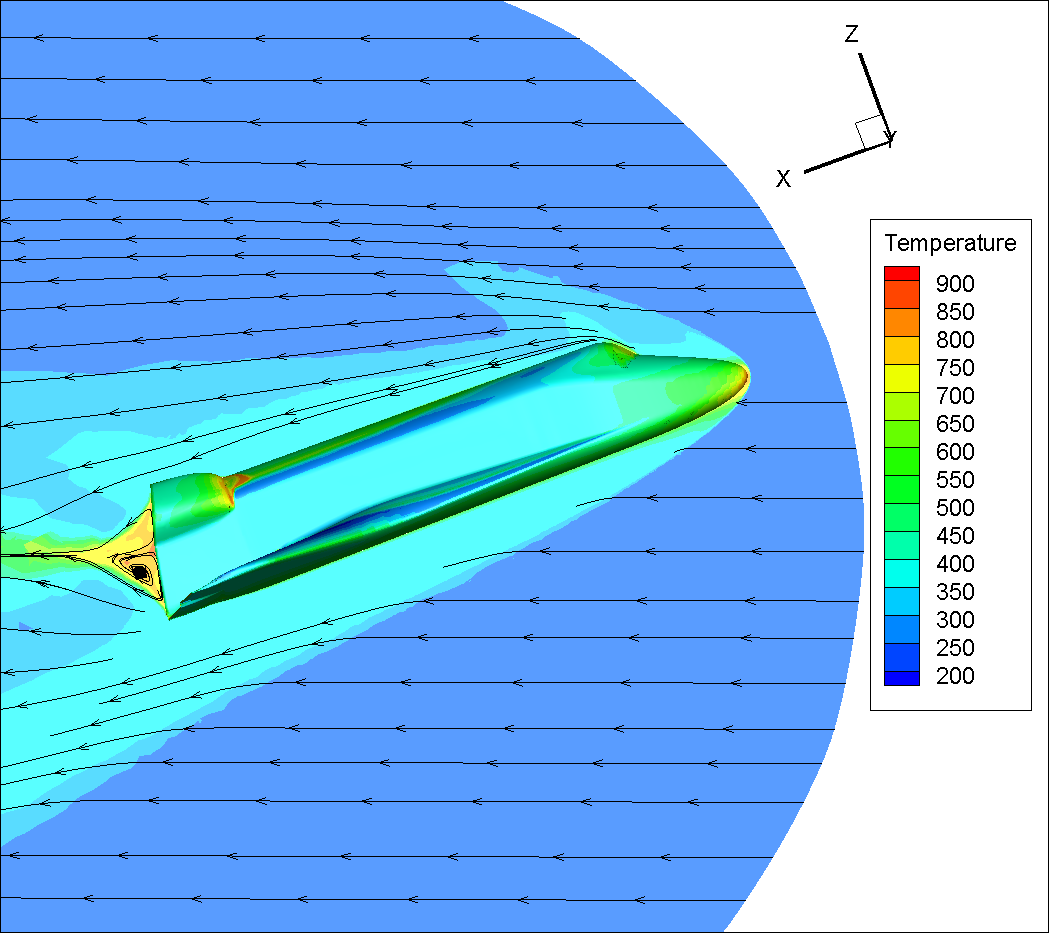
\includegraphics[width=\textwidth]{report_images/20_adapted_sym_temp_contour.png}
		 \caption{Temperature contour at the midspan of the wing of the orbiter at 20 degs AoA using adapted grid}
		 \label{fig: 20_adapt_sym_temp_contour}
    \end{subfigure}
%	\caption{Caption place holder}  
\end{figure}

\begin{figure}[H]

	\centering
    \begin{subfigure}[b]{0.65\textwidth}
         \centering
		 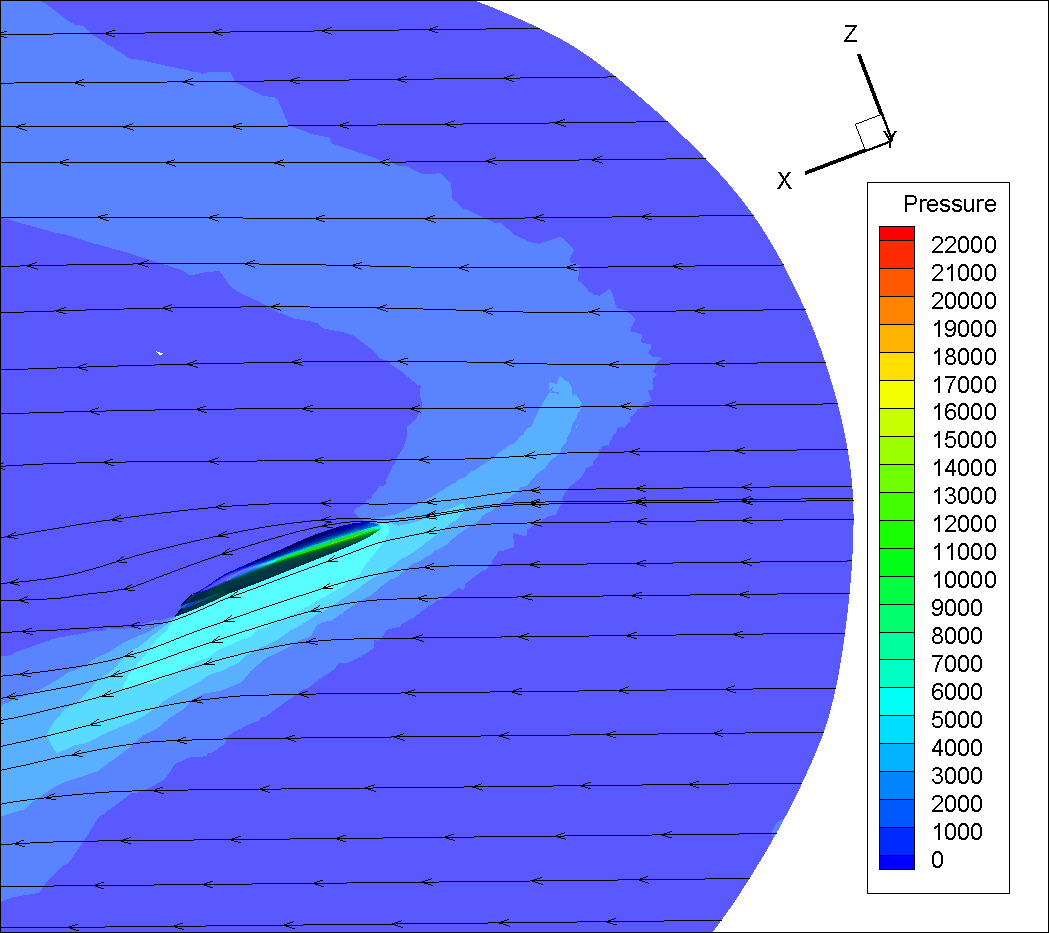
\includegraphics[width=\textwidth]{report_images/20_wing_pressure_contour.png}
		 \caption{Pressure contour at the midspan of the wing of the orbiter at 20 degs AoA}
		 \label{fig: 20_wing_pressure_contour}
    \end{subfigure} 
    \begin{subfigure}[b]{0.65\textwidth}
         \centering
		 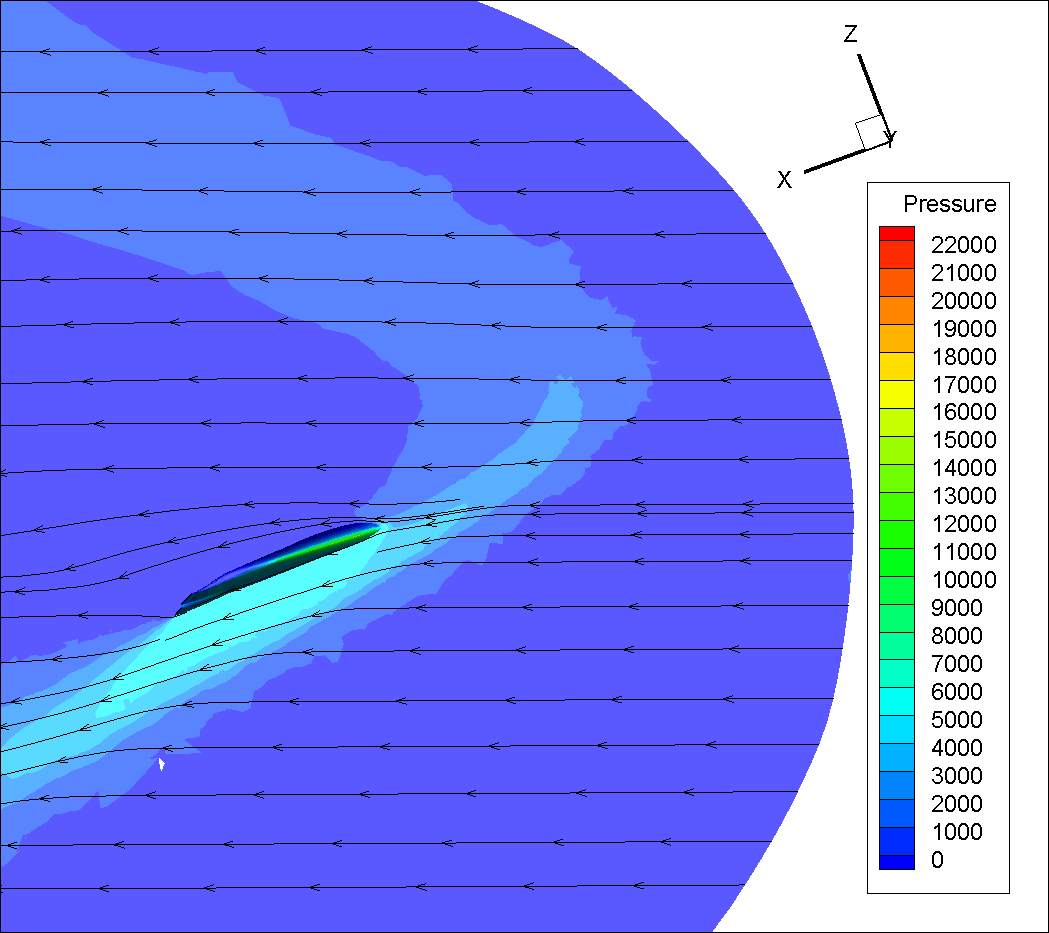
\includegraphics[width=\textwidth]{report_images/20_adapted_wing_pressure_contour.png}
		 \caption{Pressure contour at the midspan of the wing of the orbiter at 20 degs AoA using adapted grid}
		 \label{fig: 20_adapt_wing_pressure_contour}
    \end{subfigure}
\end{figure}

\begin{figure}[H]

	\centering
    \begin{subfigure}[b]{0.65\textwidth}
         \centering
		 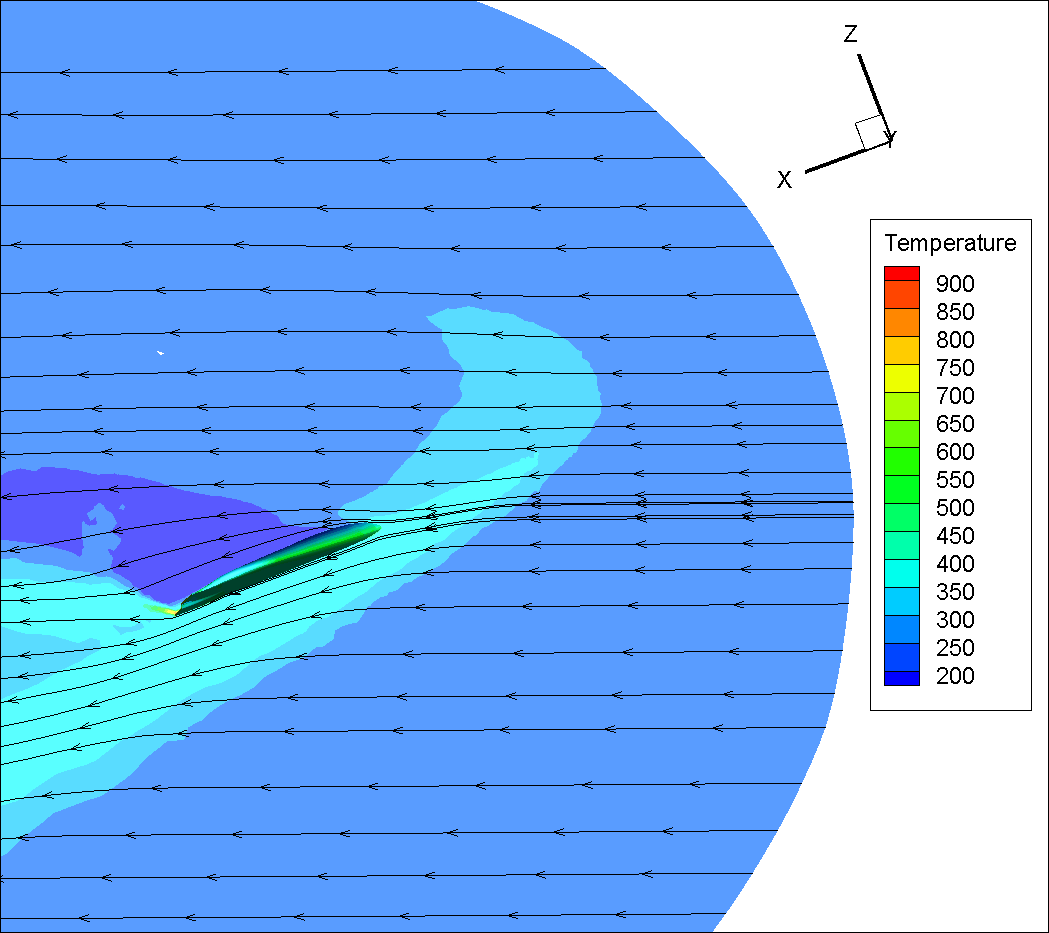
\includegraphics[width=\textwidth]{report_images/20_wing_temp_contour.png}
		 \caption{Temperature contour at the midspan of the wing of the orbiter at 20 degs AoA}
		 \label{fig: 20_wing_temp_contour}
    \end{subfigure} 
    \begin{subfigure}[b]{0.65\textwidth}
         \centering
		 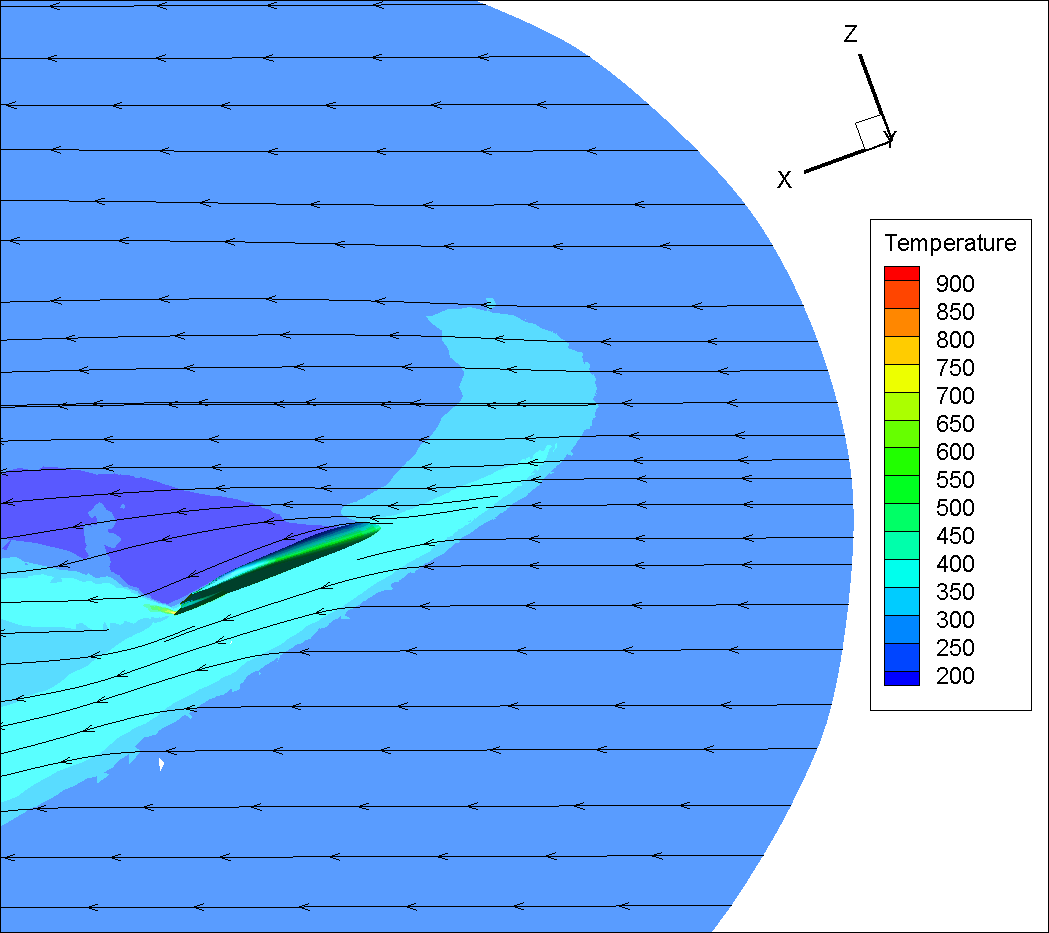
\includegraphics[width=\textwidth]{report_images/20_adapted_wing_temp_contour.png}
		 \caption{Temperature contour at the midspan of the wing of the orbiter at 20 degs AoA using adapted grid}
		 \label{fig: 20_adapt_wing_temp_contour}
    \end{subfigure}
%	\caption{Caption place holder}  
\end{figure}

\subsubsection{Side by side of mesh}

\begin{figure}[H]

	\centering
    \begin{subfigure}[b]{0.65\textwidth}
         \centering
		 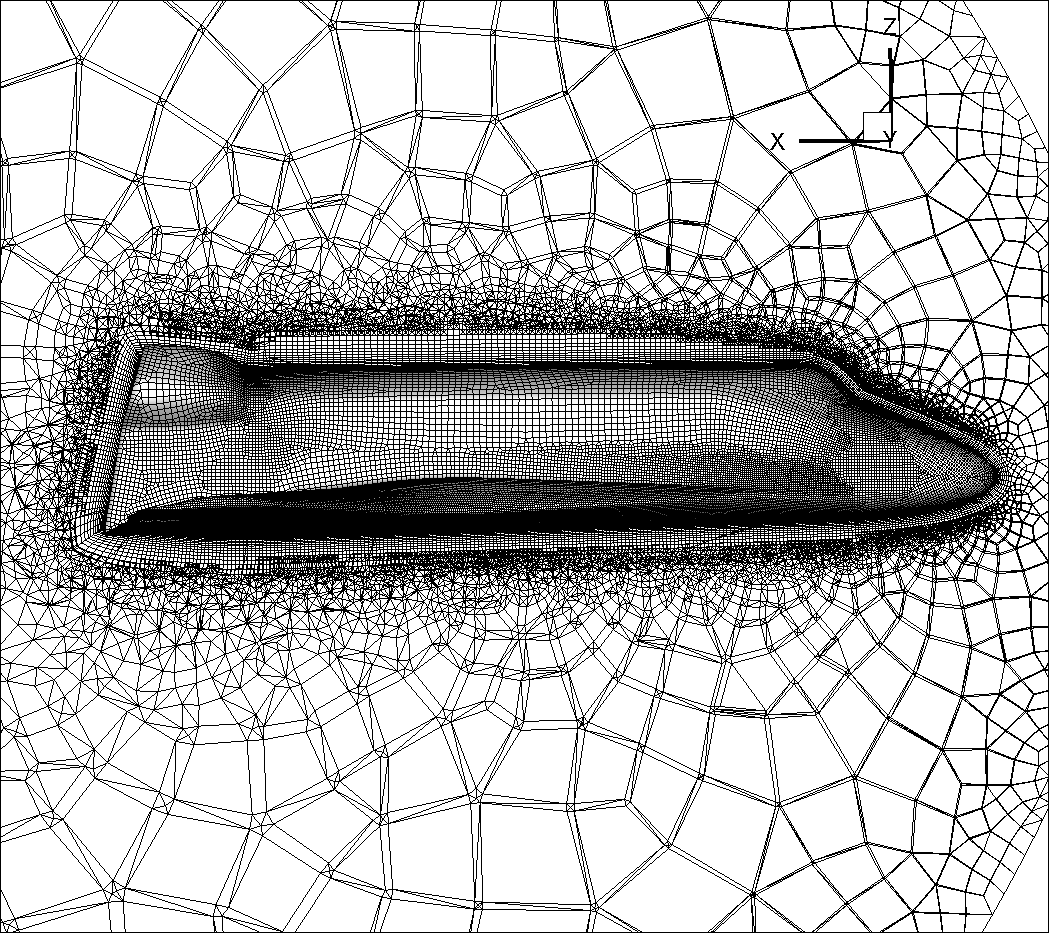
\includegraphics[width=\textwidth]{report_images/20_grid.png}
		 \caption{Grid at the symmetry plane of the orbiter at 20 degs AoA}
		 \label{fig: 20_grid}
    \end{subfigure} 
    \begin{subfigure}[b]{0.65\textwidth}
         \centering
		 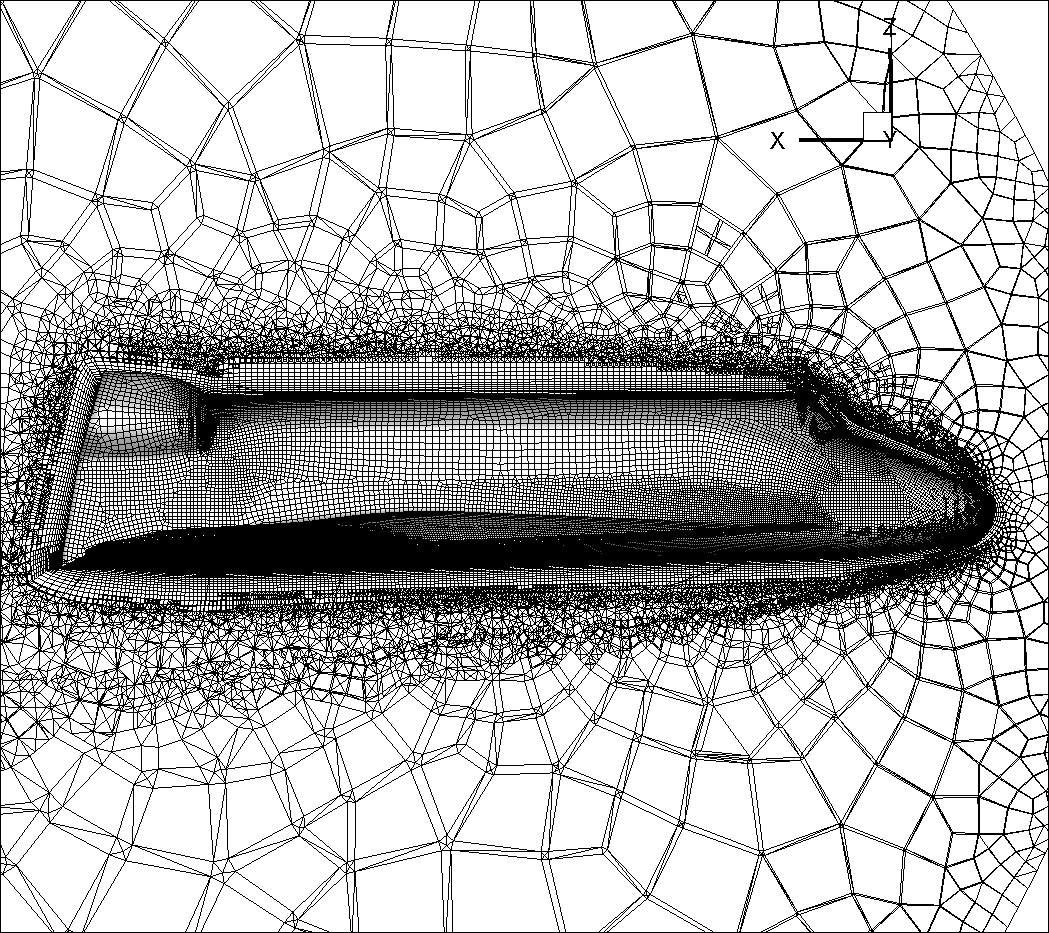
\includegraphics[width=\textwidth]{report_images/20_adapted_grid.png}
		 \caption{Adapted grid at the symmetry plane of the orbiter at 20 degs AoA}
		 \label{fig: 20_adapt_grid}
    \end{subfigure}
%	\caption{Caption place holder}  
\end{figure}

\begin{figure}[H]

	\centering
    \begin{subfigure}[b]{0.65\textwidth}
         \centering
		 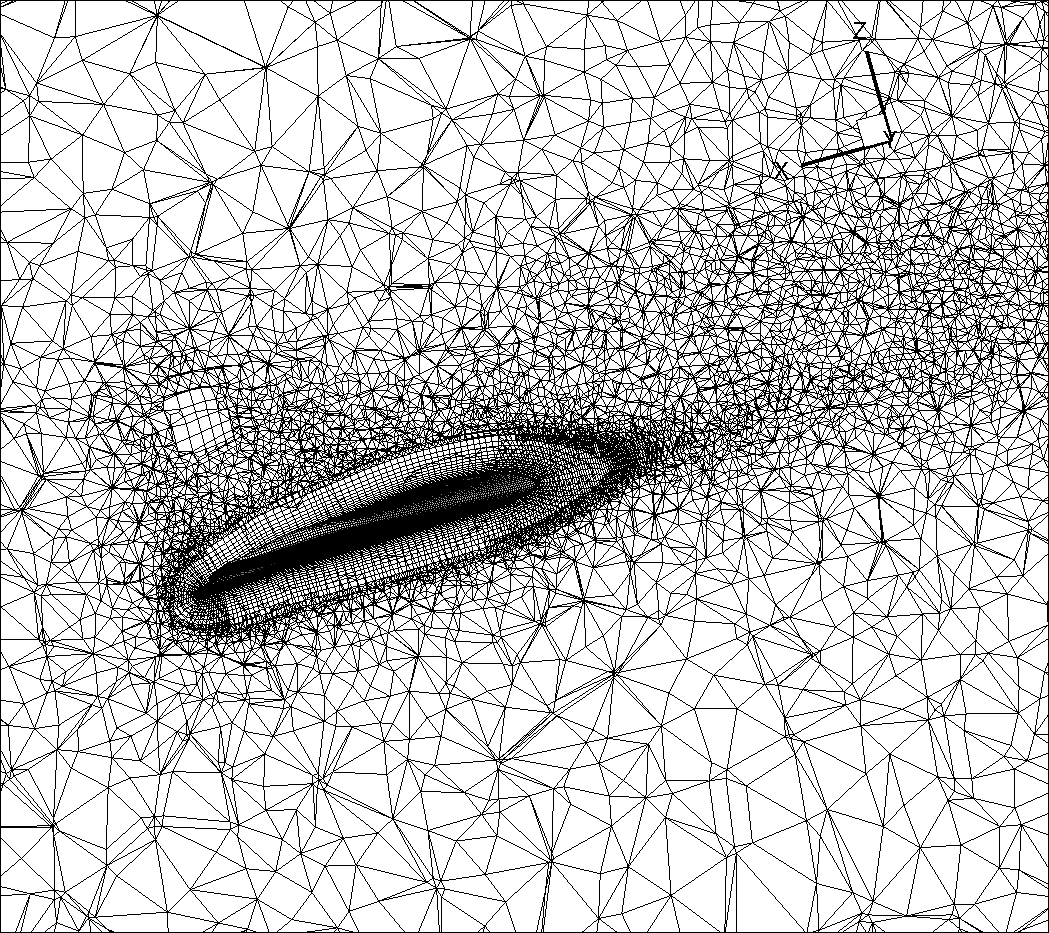
\includegraphics[width=\textwidth]{report_images/20_wing_grid.png}
		 \caption{Grid at the midspan of the wing of the orbiter at 20 degs AoA}
		 \label{fig: 20_wing_grid}
    \end{subfigure} 
    \begin{subfigure}[b]{0.65\textwidth}
         \centering
		 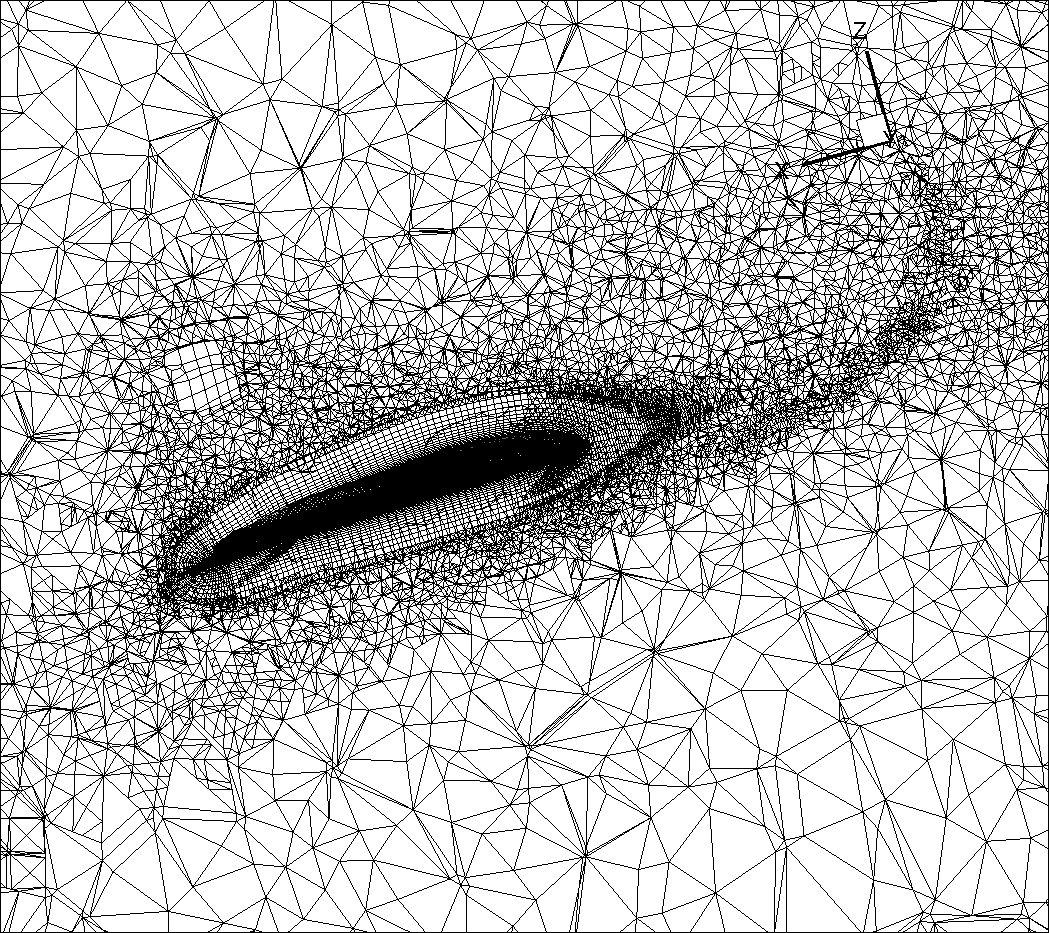
\includegraphics[width=\textwidth]{report_images/20_adapted_wing_grid.png}
		 \caption{Adapted grid at the midspan of the wing of the orbiter at 20 degs AoA}
		 \label{fig: 20_adapted_wind_grid}
    \end{subfigure}
%	\caption{Caption place holder}  
\end{figure}

\subsubsection{Table of force coefficients}
\begin{table}[H]
	\centering
	\begin{tabular}{|c|c|c|c|c|} \hline
		\centering
		\textbf{Case [$^\circ$]}       & $C_L$ [-]   & $C_D$ [-] \\ \hline
		20         & 0.341 & 0.174 \\ \hline
		Adapted 20 & 0.342 & 0.173 \\ \hline
	\end{tabular}
\end{table}
\subsubsection{Fluent settings used to adapt grid}

I forgot to keep track of what my exact settings were. However, I went back and recreated the settings based on what I remember. Admittedly, the 50\% increase in number of cells was much larger than 10\% expected. Nevertheless, even with this large increase, the differences are subtle. The most distinct difference in the mesh around the fuselage is on the "belly" of the Orbiter, while increased mesh density can be somewhat observed at the nose and turning corners of the Orbiter. The wing saw an denser mesh all around. The coefficients of lift and drag were not significantly altered. The settings of the gradient adaptations were approximately as follows, 

\begin{itemize}
	\item Options: Refine
	\item Method: Gradient
	\item Normalization: standard 
	\item Gradients of: Pressure, static pressure 
	\item Refine Threshold: ~200
	\item Max: 11,190
	\item Min: 2.588e-05
\end{itemize}


\begin{figure}[H]
     \centering
	 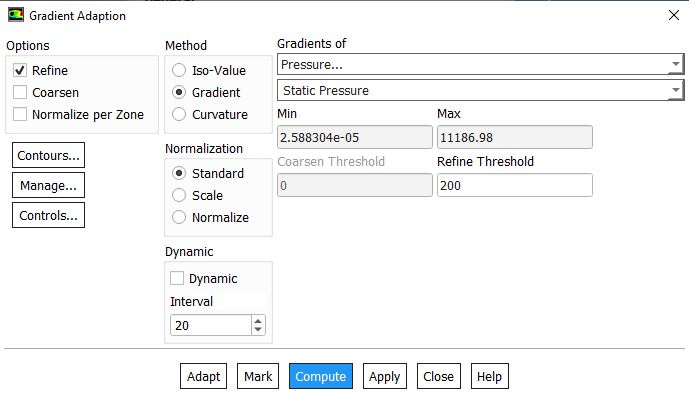
\includegraphics[width=\textwidth]{report_images/adaptation_settings.jpg}
	 \caption{Grid adaptation settings}
	 \label{fig: adapt_settings}
\end{figure}

The results of the adaptation are summarized in the screenshot below,

\begin{figure}[H]
     \centering
	 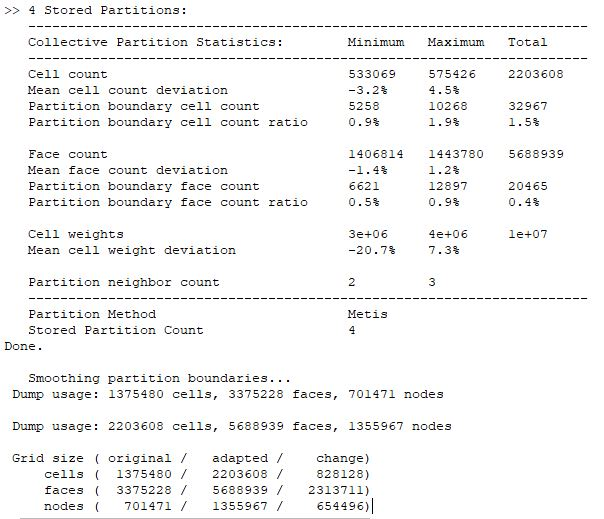
\includegraphics[width=\textwidth]{report_images/adaptation_summary.jpg}
	 \caption{Grid adaptation summary}
	 \label{fig: adapt_summary}
\end{figure}
	
